\subsection{Periodo di Avvio e di Analisi }
	\subsubsection{Periodo di Avvio (2018/12/4 - 2018/12/17)}
		Nel periodo di avvio hanno luogo le seguenti attività:
		\begin{itemize}
			\item Ricerca degli strumenti (2018/12/4 - 2018/12/14): i membri del gruppo effettuano le ricerche sui possibili strumenti utili alle attività di avvio e di analisi dei requisiti
			\item Prima normazione (2018/12/5 - 2018/12/14): gli amministratori redigono le norme di progetto concordate per i processi di supporto e organizzativi.
			\item Studio di fattibilità (2018/12/4 - 2018/12/8): gli analisti effettuano lo studio di fattibilità dei capitolati
			\item Pianificazione di progetto (2018/12/7 - 2018/12/13): il responsabile redige il piano di progetto, riportando modello di sviluppo, analisi dei rischi e la pianificazione per le prime attività dell'analisi dei requisiti
			\item Verifica dei documenti (2018/12/15 - 2018/12/16): i verificatori controllano se i documenti siano corretti
		\end{itemize}
		
	\subsubsection{Periodo di Analisi (2018/12/17 - 2018/01/21)}	
		\paragraph{Pianificazione (2018/12/17 - 2018/01/03)} Il periodo di analisi dei requisiti inizia con le attività di:
			\begin{itemize}
				\item pianificazione di progetto (2018/12/17 - 2018/12/21): il responsabile effettua il resoconto del periodo di avvio e pianifica in maniera più dettagliata le attività di analisi dei requisiti. 
				\item pianificazione della qualifica (2018/12/17 - 2018/12/21): i verificatori redigono il resoconto del periodo di avvio e i progettisti redigono i primi incrementi per il piano dei test di sistema. 
				\item normazione (2018/12/17 - 2018/12/21): gli amministratori redigono in maniera precisa e completa le norme per l'attività di analisi. 
				\item verifica dei piani e delle norme (2018/12/21 - 2018/12/23)
			\end{itemize}
		
		\paragraph{Analisi dei requisiti del sistema (2018/12/19 - 2018/01/13)} la parte centrale del periodo di analisi dei requisiti è costituita dalle attività di:
			\begin{itemize}
				\item Analisi dei Requisiti del sistema (2018/12/19 - 2018/12/27): gli analisti svolgono la prima analisi dei requisiti del sistema.
				\item Incrementi al Piano di Qualifica (2018/12/26 - 2018/12/30): i progettisti migliorano il piano dei test di sistema in base a quanto scaturito dall'analisi.
				\item Verifica dell'analisi dei requisiti di sistema (2018/12/29 - 2018/12/31)
				\item Verifica del Piano di Qualifica (2018/01/02 - 2018/01/03)
				\item Incrementi all'analisi dei requisiti (2018/01/02 - 2018/01/08): gli analisti aggiungono degli incrementi all'analisi di sistema
				\item Verifica degli incrementi all'analisi dei requisiti (2018/01/09 - 2018/01/11)
				\item Incrementi al Piano di Progetto (2018/01/07 - 2018/01/10): il responsabile redige la parte di rendicontazione e consuntivo del piano di progetto da presentare alla Revisione dei Requisiti.
				\item Incrementi al Piano di Qualifica (2018/01/07 - 2018/01/10): i verificatori redigono la parte di rendicontazione del piano di qualifica da presentare alla Revisione dei Requisiti, aggiungendo i risultati delle misurazioni effettuate.
				\item Verifica dei piani di Progetto e Qualifica (2018/01/11 - 2018/01/12)
				\item Preparazione alla presentazione (2018/01/15 - 2018/01/20)
				\item Analisi dei requisiti software (2018/02/01 - 2018/02/05): gli analisti effettuano l'analisi dei requisiti software. Quest'attività è successiva al primo incremento di progettazione architetturale.
				\item Verifica dell'analisi dei requisiti (2018/02/07 - 2018/02/09)				
			\end{itemize}
	\newpage
	\begin{figure}[!hbtp]
		\centering
		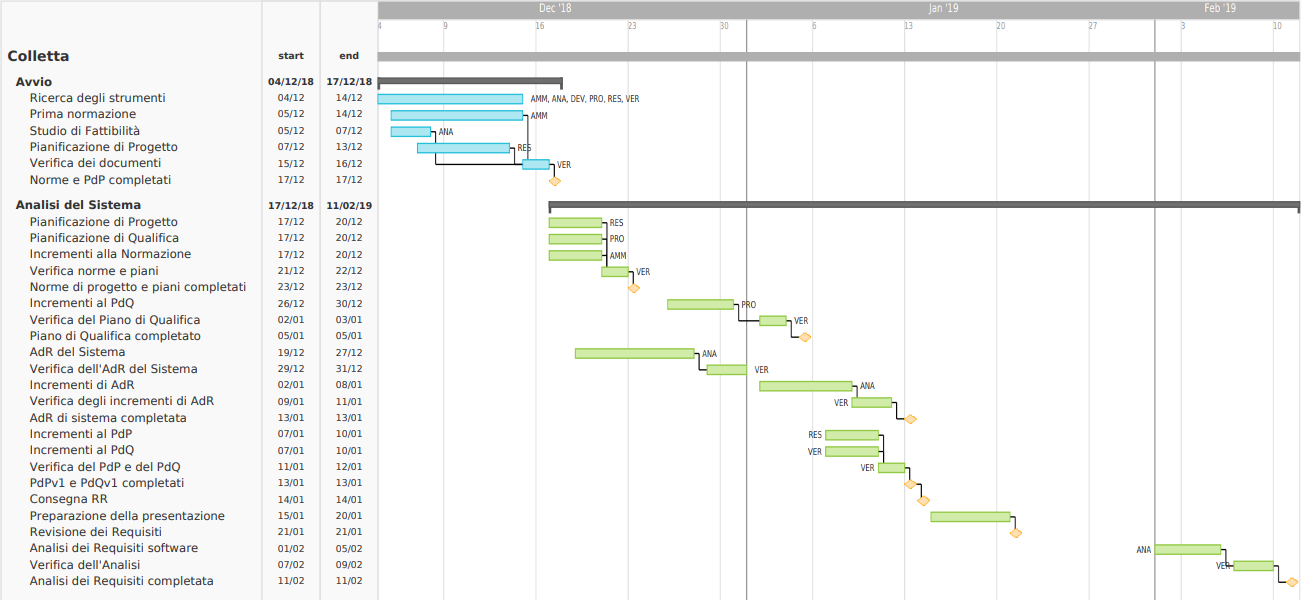
\includegraphics[scale=0.5,angle=90]{images/gantt.png}
		\caption{Diagramma di Gantt per il periodo di avvio e di analisi}
	\end{figure}
	\newpage